\documentclass[11pt, oneside]{article}   	% use "amsart" instead of "article" for AMSLaTeX format
\usepackage{geometry}                		% See geometry.pdf to learn the layout options. There are lots.
\geometry{letterpaper}                   		% ... or a4paper or a5paper or ... 
\usepackage{graphicx}				% Use pdf, png, jpg, or eps§ with pdflatex; use eps in DVI mode
								% TeX will automatically convert eps --> pdf in pdflatex		
\usepackage{amssymb}
\usepackage{amsmath}
\usepackage{parskip}
\usepackage{color}
\usepackage{hyperref}

\graphicspath{{/Users/telliott_admin/Dropbox/Tex/png/}}
% \begin{center} 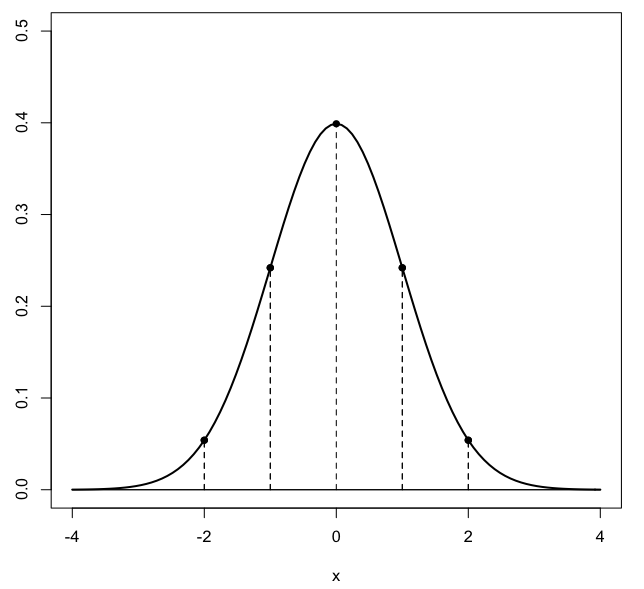
\includegraphics [scale=0.4] {gauss3.png} \end{center}

%break
\title{Riemann sums with graduated intervals}
\date{}

\begin{document}
\maketitle
\Large

\subsection*{intervals of unequal width}
Courant and John describe a variation on Riemann sums using intervals of unequal (but graduated) width.  This "trick" allows them to derive the formula for 
\[ \int x^n \ dx = \frac{x^{n+1}}{n+1} \]
\[ \int_a^b x^n \ dx = \frac{b^{n+1} - a^{n+1}}{n+1} \]
for all natural numbers $n$ first, and then with some elaborations, for real $n$ except $n = -1$.

\subsection*{Fermat version}
I found a simple proof on the web, due to Fermat.

\url{http://fredrickey.info/hm/CalcNotes/Fermat-Integration.pdf}

It is really the basis for the Courant and John proof.  It achieves simplicity by using the interval $[0,b]$ with its lower bound at zero.

Let $E$ be a positive constant less than $1$.  Divide the region $[0,b]$ into subintervals with boundaries 
\[ \dots bE^3, bE^2, bE, b \]

How do we get the number of rectangles to increase to infinity?  By letting $E \rightarrow 1$ and taking the limit.

Construct rectangles in the usual way that circumscribe the curve $y = x^n$ and add up their areas.  For the $i$th rectangle, the width is
\[ bE^i - bE^{i+1} \]
($bE^{i+1} < bE^i$), and the height is
\[ (bE^i)^n \]
so the overall sum is
\[ S = \sum_{i = 0}^{\infty} (bE^i)^n \ (bE^i - bE^{i+1}) \]
\[ = b^{n+1} \sum_{i = 0}^{\infty} (E^i)^n \ (E^i - E^{i+1}) \]
\[ = b^{n+1} \sum_{i = 0}^{\infty} (E^i)^{n+1} \ (1 - E) \]
\[ = b^{n+1} \ (1 - E) \ \sum_{i = 0}^{\infty} (E^{n+1})^i \]

Since $E$ is a positive constant less than $1$, $E^{n+1}$ is also.  Let $q = E^{n+1}$.  The sum becomes
\[ \sum_{i = 0}^{\infty} q^i = q^0 + q^1 + q^2 + q^3 + \dots \]
Recall that
\[ \frac{1}{1-x} = 1 + x + x^2 + x^3 + \dots \]
for $|x| < 1$.  

So, going back to $E$ we have
\[ S = b^{n+1} \ (1 - E) \ \frac{1}{1 - E^{n+1}} \]
and using the same identity again
\[ 1 - x = \frac{1}{1 + x + x^2 + x^3 + \dots } \]
so
\[ S = b^{n+1} \ \frac{1}{(1 + E + E^2 + E^3 + \dots)(1 - E^{n+1})} \]
All the terms in the infinite series starting at $E^{n+1}$ acquire counterparts with a minus sign, hence
\[ = b^{n+1} \ \frac{1}{1 + E + E^2 + E^3 + \dots + E^n} \]

Now take the limit as $E \rightarrow 1$.  The fraction becomes just
\[ \frac{1}{1 + E + E^2 + E^3 + \dots + E^n}  = \frac{1}{n+1} \]
and we have
\[ \int_0^b x^n = \frac{b^{n+1}}{n+1} \]
which is what we get when we evaluate $x^{n+1}$ on the interval $[0,b]$ and then divide by $n+1$.

\end{document}